\documentclass[a4paper,11pt]{article}

\usepackage[spanish,activeacute]{babel}
\usepackage[utf8]{inputenc}
\usepackage[dvipdfm]{graphicx}
\usepackage{amssymb,amsmath}
\usepackage{fancyvrb}
\usepackage{enumerate}
%\usepackage{pseudocodees}
\usepackage{indentfirst}
\usepackage{multirow}
\usepackage{color}

\usepackage[a4paper, margin=2.5cm, top=2cm, bottom=3cm]{geometry}

\pagestyle{empty}

\definecolor{lightgray}{rgb}{1, 1, 1}
\newcommand{\light}[1]{\textcolor{lightgray}{#1}}
\definecolor{hidden}{rgb}{1, 1, 1}
\newcommand{\hidden}[1]{\textcolor{hidden}{#1}}

\begin{document}


\begin{center}
\begin{tabular}{p{5.2cm}r}
\multirow{5}{*}[0.35cm]{\scalebox{0.18}{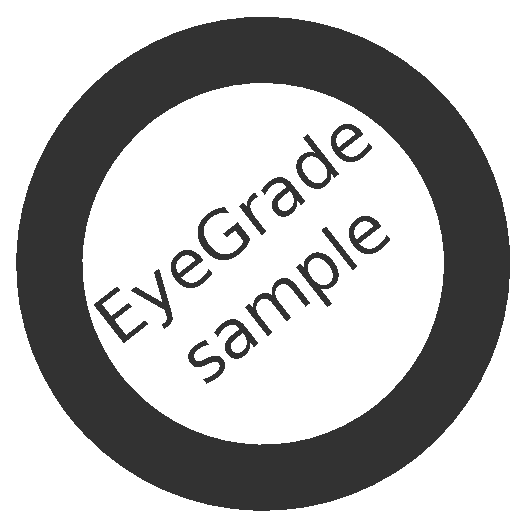
\includegraphics{sample-logo.eps}}} &
\Large  \textbf{{{subject}}} \\
& \textbf{{{degree}}} \\
& \\
Leganés, {{date}}
      & {{title}}. \\
Duration: {{duration}}
      & Score: 5 points out of 10 total points for the exam. \\

\end{tabular}
\end{center}

\vspace{0.5cm}


\emph{There is only one correct answer for each multiple choice question.
Each correct answer adds $\frac{1}{4}$ points. 
Each incorrect answer has a penalty of $\frac{1}{12}$ points.
If no answer no score is awarded, neither positive nor negative.}

\vspace{0.5cm}

\begin{center}
\begin{tabular}{|p{0.8\textwidth}|}
\hline
\begin{itemize}
\item Mark out your answers with an ``X''.
\item If more than one answer or no answer are selected, the question is considered to be not answered (no score is awarded, neither positive nor negative).
\item Fill in \textbf{all the fields} of the following form.
% \item Be especially careful with the \textbf{model of exam}: if you write
%   a wrong model identifier, your score will be random.
%   If you don't write the model identifier, your score will be 0.
\end{itemize}
\\

\hline
\end{tabular}
\end{center}

\vspace{0.2cm}


\begin{center}
(1) Write your personal data clearly. 
\end{center}

\begin{center}
\large

\begin{tabular}{|l|p{12cm}|}
\hline
Last name:   &  \\
\hline
First name: &    \\
\hline
Group:   &  \\
\hline
\end{tabular}
\end{center}

\vspace{0.2cm}

\begin{center}
(2) Write down your NIA and cross out your answers with an ``X'' mark:
\end{center}

\begin{center}
\large
\textbf{Model:} {{model}}
\end{center}

{{id-box(9,NIA)}}

{{answer-table}}

\clearpage

{{questions}}

\end{document}
